%---------- Sexto Capítulo: Resultados ----------
\chapter{Resultados}
\label{chap:result}
% TODO: introduzir a seção de resultados
O último passo presente em todo projeto é a análise dos resultados obtidos, ou seja, quais foram os produtos de todo o processo de desenvolvimento e se os mesmos estão com qualidade dentro do esperado no início do processo. 

O capítulo é dividido em três subseções: Metodologia Empregada (seção \ref{sec:metod}), Performance do Sistema (seção \ref{sec:perf}) e Considerações (seção \ref{sec:consid}). A primeira consiste numa análise dos resultados obtidos ao se empregar a metodologia definida no capítulo \ref{metod}, como verificar se a mesma se mostrou eficiente através da análise de estatísticas de rendimento coletadas ao longo do projeto. A segunda mostra o estudo feito em relação a performance do sistema desenvolvido, principalmente quanto ao tempo de resposta do mesmo a requisições concorrentes. Por fim é realizada na última seção uma crítica quanto aos resultados alcançados no processo de desenvolvimento do presente projeto.

\section{Metodologia Empregada}
\label{sec:metod}
% TODO: escrever texto e referencias as figuras
Como anteriormente apresentado no capítulo \ref{metod}, a metodologia empregada baseou-se em distribuir o processo de desenvolvimento do \emph{software}, com o objetivo de acelerar este processo, permitindo ao mesmo tempo que a equipe fosse capaz de trabalhar de forma distribuída, sendo necessário reuniões periódicas para discussão de novas funcionalidades e refatoramento do código.

Entre os resultados da metodologia empregada, estão estatísticas que indicam o número de linhas de código criadas por cada programador.
A figura \ref{fig:linesofcode} apresenta um gráfico do número de linhas de código do projeto em função do tempo.
A partir deste gráfico, observa-se que o processo de codificação foi realizado entre o dia 14 de Julho e o dia 25 de Outubro de 2011, totalizando cerca de 6000 linhas de código.
O maior salto de produtividade aconteceu durante o período de 24 de Julho e 9 de Agosto, período no qual foram criadas e implementadas grande parte das entidades do \emph{Core} do sistema.
Neste mesmo período, foram também realizados refatoramentos no código, resultando no rápido crescimento de linhas de código escritas que pode ser visto através do gráfico.

\begin{figure}[!htb]
	\centering
	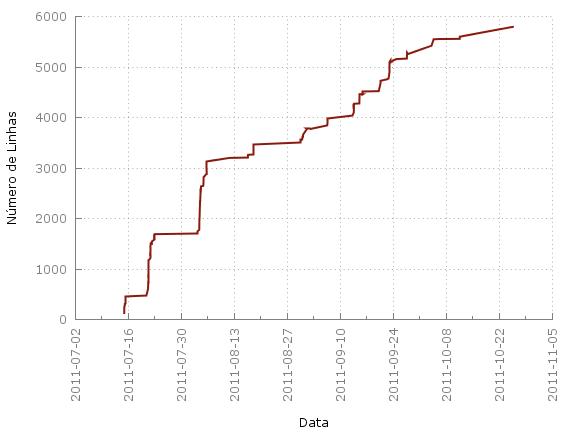
\includegraphics[width=0.7\textwidth]{./plots/lines_of_code.png}
	\caption[Evolução do número de linhas de código do projeto]{Evolução do número de linhas de código do projeto ao longo do processo de desenvolvimento}
	\fonte{Autoria Própria}
	\label{fig:linesofcode}
\end{figure}

Através do histórico dos \emph{commits} feitos com as contas de cada programador no sistema de controle de versão, foi possível também estimar a contribuição, em linhas de código, de cada desenvolvedor.
A figura \ref{fig:linesofcodebyauthor} apresenta um gráfico que relaciona o numéro de linhas de código contribuídas por cada desenvolvedor ao longo do tempo.
Vale notar que estes valores são cumulativos, ou seja, mesmo que uma linha criada por um programador tenha sido deletada, esta continua sendo levada em conta como uma linha escrita pelo programador que a criou.

% TODO: tirar mais conclusões desse gráfico, talvez explicar que algumas integrações e refatoramentos grandes do projeto foram feitas em conjunto, mas commitadas com a minh a conta

\begin{figure}[!htb]
	\centering
	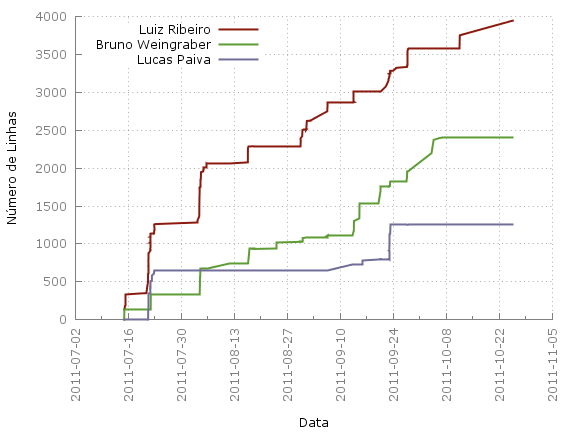
\includegraphics[width=0.7\textwidth]{./plots/lines_of_code_by_author.png}
	\caption[Evolução do número de linhas de código por programador]{Evolução do número de linhas de código do projeto por programador ao longo do processo de desenvolvimento}
	\fonte{Autoria Própria}
	\label{fig:linesofcodebyauthor}
\end{figure}

As figuras \ref{fig:dayofweek} e \ref{fig:hourofday}, por sua vez, apresentam estatísticas com relação ao número de \emph{commits} no sistema de controle de versão em função do dia da semana e do horário.
Através destes gráficos é possível notar que, graças à característica de desenvolvimento distribuído da metologia empregada, o processo de codificação aconteceu durante vários horários distintos: mesmo que um desenvolvedor não fosse capaz de trabalhar em um determinado horário, muito provavelmente outro seria, resultando em um impacto positivo sobre o rendimento do processo de desenvolvimento.

\begin{figure}[!htb]
	\centering
	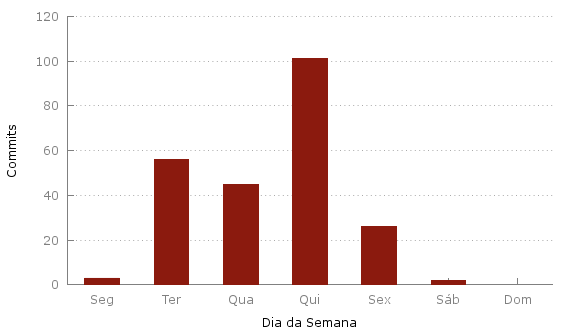
\includegraphics[width=0.7\textwidth]{./plots/day_of_week.png}
	\caption[Número de \emph{commits} por dia da semana]{Número de \emph{commits} por dia da semana}
	\fonte{Autoria Própria}
	\label{fig:dayofweek}
\end{figure}

\begin{figure}[!htb]
	\centering
	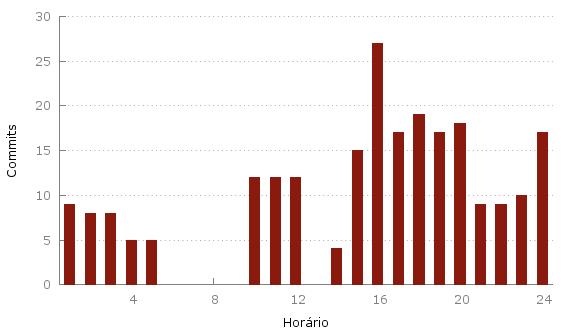
\includegraphics[width=0.7\textwidth]{./plots/hour_of_day.png}
	\caption[Número de \emph{commits} por horário]{Número de \emph{commits} por horário}
	\fonte{Autoria Própria}
	\label{fig:hourofday}
\end{figure}

Aliada à arquitetura modular que foi proposta para o \emph{software}, esta metodologia mostrou-se eficiente ao longo do projeto, tendo em vista que muitas vezes os horários dos integrantes da equipe eram incompatíveis entre si, sendo de grande importância a possibilidade dos mesmos trabalharem de forma independente.
Além disso, a escolha de ferramentas como, por exemplo, o uso do sistema de controle de versão git e do serviço de hospedagem de repositórios GitHub, reforçaram ainda mais a metodologia empregada, já que tais ferramentas forneceram meios para estabelecimento de metas e estatísticas de desempenho de cada desenvolvedor, técnicas fundamentais para acompanhar o desenvolvimento do projeto e o rendimento da equipe.

\section{Performance do Sistema}
\label{sec:perf}
Como métrica para analisar a performance do sistema, optou-se por utilizar testes de \emph{stress} no \emph{Web Service}, ou seja, executar uma série de consultas simultaneamente e avaliar o impacto no tempo de resposta do mesmo.

Para tanto, foram realizados testes com o auxílio da ferramenta ApacheBench \cite{apachebench}.
Os testes foram executados em um único servidor com processador Intel{\textsuperscript\textregistered} Xeon{\textsuperscript\textregistered} X3450 de 2.67GHz e 2GB de memória RAM.
O servidor HTTP utilizado para hospedar a aplicação foi o Jetty, assim como descrito no Apêndice \ref{ape:guia}.

Tendo em vista a dificuldade que a equipe teve de obter informações de transporte público para cidades brasileiras, todos os testes utilizaram a base de dados do Bay Area Rapid Transit (BART), da cidade de São Francisco, Califórnia.
Esta base de dados é composta por 48 \emph{Stops}, 13 \emph{Routes}, cerca de 30 mil \emph{StopTimes} e 1500 \emph{Trips}.
% TODO: esse é o melhor jeito de dizer o tamanho da base de dados usada?

Foram executados cinco testes, sendo cada um destes composto por 1000 requisições.
O primeiro dos testes correspondeu à execução de todas as requisições sequencialmente, uma por segundo.
O segundo dos testes foi realizado com duas requisições concorrentes por segundo e, os demais testes, foram compostos por 5, 10 e 20 requisições por segundo.
O impacto do aumento do número de requisições concorrentes pode ser acompanhado através da Figura \ref{fig:response}, a qual apresenta o tempo de resposta para cada uma das requisições feitas nos testes descartando a latência da rede.

\begin{figure}[!htb]
	\centering
	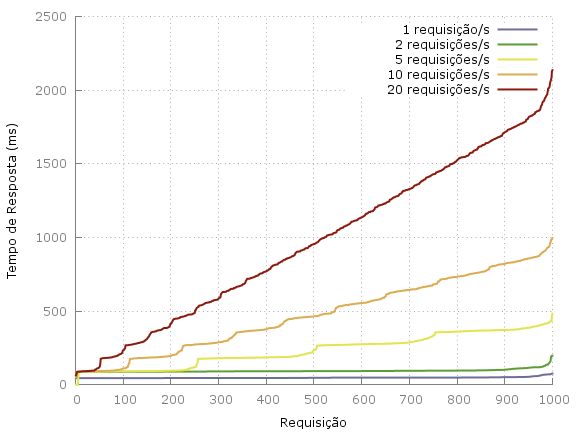
\includegraphics[width=0.7\textwidth]{./plots/stresstests/out.png}
	\caption[Tempo de resposta do \emph{Web Service}]{Tempo de resposta do \emph{Web Service} em função do número de requisições}
	\fonte{Autoria Própria}
	\label{fig:response}
\end{figure}

A partir do gráfico apresentado na Figura \ref{fig:response} é possível notar que, sob as condições propostas para o experimento, o serviço foi capaz de atender todas as requisições sequenciais em menos de 100 ms.
No teste de 2 requisições concorrentes por segundo, o serviço foi capaz de atender todas as requisições em menos de 200ms.
Para os testes de 5, 10 e, principalmente, 20 requisições concorrentes por segundo, as últimas requisições tiveram um tempo de resposta significativo, sendo em alguns casos necessários pouco mais de 2 segundos para responder a requisição de um cliente.

Apesar da aparente ruim performance no teste com 20 requisições concorrentes, deve-se levar em conta que para este teste foi utilizado apenas um servidor.
Para melhorar a performance do sistema em um ambiente com uma grande quantidade de requisições concorrentes, é possível utilizar diversos servidores e utilizar um mecanismo de escalonamento, de forma que as requisições sejam alocadas aos servidores que possuem mais tempo de CPU livre no momento, consequentemente minimizando o tempo de resposta.
Vale notar também que o caso de 20 requisições por segundo é um teste de \emph{stress} do sistema, o que não corresponde necessariamente à um caso de uso real.

\section{Considerações}
\label{sec:consid}
A metodologia idealizada só foi possível de ser empregada devido a característica modular do sistema, visto que proporcionou o desenvolvimento paralelo pelos integrantes da equipe.
Geralmente os horários dos mesmos eram incompatíveis e, desta forma se outra metodologia que exigisse reuniões frequentes fosse utilizada, o desenvolvimento teria sido ineficiente.
Aliado a este fator estão as técnicas de gerência de projeto, como estabelecimento de metas e análise de desempenho por desenvolvedor, possíveis somente devido ao uso das ferramentas como o sistema controlador de versão git juntamente com o site de hospedagem de repositório Github.

Quanto ao desempenho do sistema como um todo, deve-se ressaltar o uso de somente um servidor para a coleta das estatísticas de performance quanto ao tempo de resposta de requisições concorrentes.
Para o caso de 20 requisições por segundo aparentemente este tempo pode ser considerado alto, porém vale lembrar que este é somente um teste de estresse do sistema, não considerando necessariamente um caso real. Contudo, para empregar o sistema futuramente considera-se a utilização de mais servidores para atender a demanda dos usuários, aliada a um sistema de escalonamento com o intuito de distribuir as requisições entre os mesmos de acordo com suas respectivas taxas de ocupação da CPU.